\documentclass[tikz, border=2pt]{standalone}
\usepackage{tikz}
\usetikzlibrary{arrows.meta}
\begin{document}
    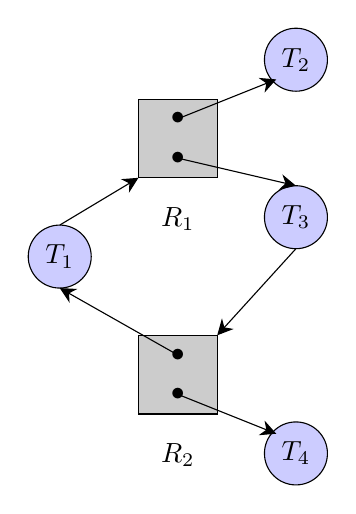
\begin{tikzpicture}
        \draw[fill=black!20] (0,0) rectangle ++(1,1) node [midway, below, yshift=-0.75cm] {$R_2$}
            node at (0.5,0.75) {$\bullet$}
            node at (0.5,0.25) {$\bullet$};
        \draw[fill=black!20] (0,3) rectangle ++(1,1) node [midway, below, yshift=-0.75cm] {$R_1$}
            node at (0.5,3.75) {$\bullet$}
            node at (0.5,3.25) {$\bullet$};
        \draw[fill=blue!20] (-1,2) circle (0.4) node {$T_1$};
        \draw[fill=blue!20] (2,2.5) circle (0.4) node {$T_3$};
        \draw[fill=blue!20] (2,4.5) circle (0.4) node {$T_2$};
        \draw[fill=blue!20] (2,-0.5) circle (0.4) node {$T_4$};
        \draw[-{Stealth[length=2mm, width=2mm]}] (2,2.1) -- (1,1);
        \draw[-{Stealth[length=2mm, width=2mm]}] (0.5,0.25) -- (1.75,-0.25);
        \draw[-{Stealth[length=2mm, width=2mm]}] (0.5,3.75) -- (1.75,4.25);
        \draw[-{Stealth[length=2mm, width=2mm]}] (-1,2.4) -- (0,3);
        \draw[-{Stealth[length=2mm, width=2mm]}] (0.5,0.75) -- (-1,1.6);
        \draw[-{Stealth[length=2mm, width=2mm]}] (0.5,3.25) -- (2,2.9);
    \end{tikzpicture}
\end{document}